\chapter{Introduction}

\section{Motivation}
Despite the advent of increasingly faster GPUs with smaller teraFLOP to price
ratios and serverless cloud GPU services, training reinforcement learning
algorithms remains an extremely time-consuming and expensive process.

Recent developments in the reinforcement learning space have helped combat
this, with more efficient algorithms such as Twin Delayed DDPG
\cite{fujimoto2018addressing} and Soft Actor-Critic \cite{haarnoja2018soft}.
However, the research has been less focused on domain specific optimizations.
This project aims to complement the generalized successes in this field, by
optimizing agent performance in specialized environments. Hopefully, the
learnings from this project can be extrapolated to other areas of knowledge.

\section{Objectives}

We recreate and optimize two model-free deep reinforcement learning techniques;
a value based method, the deep Q-network (DQN), and a hybrid\footnote{Hybrid
  method refers to algorithms that use both value based and policy based
  components} method, advantage actor-critic (A2C).

The primary objective of this project is to reduce training time while
simultaneously improving model performance in racing game environments of
varying complexity, benchmarked against the model scores from the original
papers using the DQN algorithm for each of the chosen games. We choose this
evaluation strategy to effectively compare the improvements that environment
specific optimizations can bring.

A secondary objective is to create a graphical user interface to visualize the
neural network, and its evolution as training progresses, while also allowing
the user to see gameplay. This is meant to be used as an aid to the
experimentation process, helping to optimize the chosen hyperparameters through
a visual medium and serve as an indication for suboptimal hyperparameter
selection; it is evaluated by its capability to do so.

\newpage

The main features of the project are:

\begin{itemize}
  \item Agents that use the game's observation space\footnote{Direct game data in the
          case of Mountain Car and pixels in the case of Car Racing} as inputs, and
        produce an appropriate action as the output.
  \item The agents improving at the games by training the models, without any external
        inputs or prior knowledge.
  \item A graphical user interface showcasing the gameplay, the models' performance,
        and the models' change as training progresses.
\end{itemize}

\section{Environments}

Racing games provide challenging conditions for reinforcement learning
algorithms, due to the high-dimensional input space and the need for fast and
intentional decision-making logic, especially as the game's complexity
increases. This makes them ideal as the basis of testing for the algorithms
used in this project.

Two racing games were chosen to implement the reinforcement learning
algorithms, Mountain Car and Car Racing. \autoref{fig:game_frames} shows a
frame from both of the games. Further details about the mechanics and physics
of the games are described in \autoref{sec:mountain_car_background} and
\autoref{sec:car_racing_background}.

\begin{figure}[H]
  \centering
  \begin{subfigure}{0.45\linewidth}
    \fbox{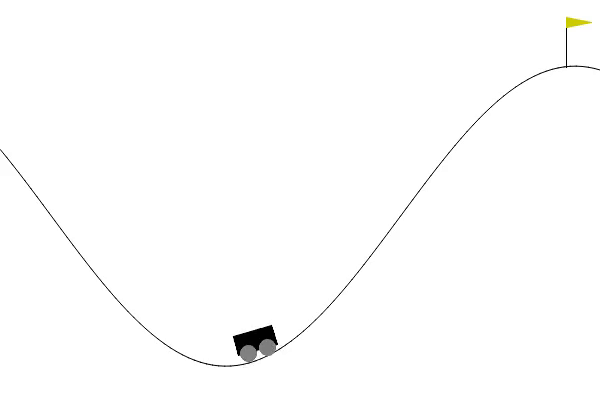
\includegraphics[height=4.5cm]{figures/images/mountain_car_frame.png}}
    \caption{Mountain Car}
  \end{subfigure}
  \hfill
  \begin{subfigure}{0.45\linewidth}
    {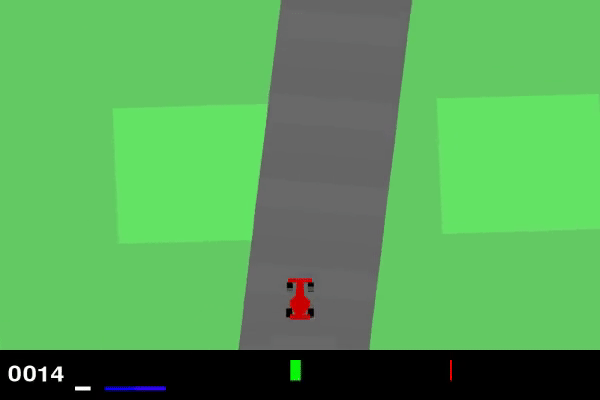
\includegraphics[height=4.5cm]{figures/images/car_racing_frame.png}}
    \caption{Car Racing}
  \end{subfigure}
  \caption[Frame from both environments]{Single frame from both of the chosen environments}
  \label{fig:game_frames}
\end{figure}


\newpage

\section{Report Structure}
The report is structured as follows:

\begin{itemize}
  \item \textbf{Background} -- discussing essential history and knowledge pertaining to the topics relevant to the project
  \item \textbf{Design \& Implementation} -- exploring the theory and reasoning behind implementation decisions, and outlining the development details of the code
  \item \textbf{Experimentation \& Evaluation} -- comparing and analysing the experimentation techniques and hyperparameters used, and examining the final results obtained
  \item \textbf{Conclusion} -- briefly summarizing the project, outlining its achievement and limitations, and exploring potential future research
\end{itemize}
